\documentclass[tikz,border=8pt]{standalone}
\usepackage{tikz}
\usetikzlibrary{positioning,arrows.meta,calc}

\begin{document}
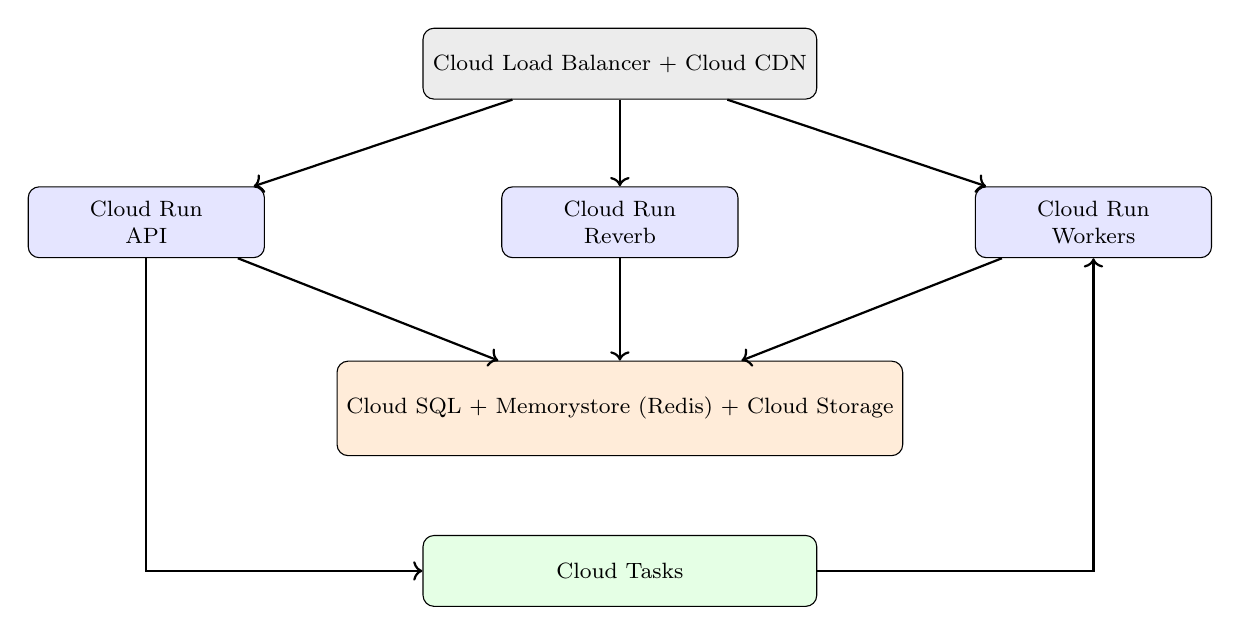
\begin{tikzpicture}[node distance=1.5cm, every node/.style={font=\footnotesize, align=center}]
    \node (cdn) [draw, rounded corners, fill=gray!15, minimum width=5cm, minimum height=0.9cm] {Cloud Load Balancer + Cloud CDN};
    \node (api) [draw, rounded corners, fill=blue!10, minimum width=3cm, minimum height=0.9cm, below left=1.1cm and 2.0cm of cdn] {Cloud Run\\API};
    \node (reverb) [draw, rounded corners, fill=blue!10, minimum width=3cm, minimum height=0.9cm, below=1.1cm of cdn] {Cloud Run\\Reverb};
    \node (workers) [draw, rounded corners, fill=blue!10, minimum width=3cm, minimum height=0.9cm, below right=1.1cm and 2.0cm of cdn] {Cloud Run\\Workers};
    \node (shared) [draw, rounded corners, fill=orange!15, minimum width=6cm, minimum height=1.2cm, below=1.3cm of reverb] {Cloud SQL + Memorystore (Redis) + Cloud Storage};
    \node (tasks) [draw, rounded corners, fill=green!10, minimum width=5cm, minimum height=0.9cm, below=1.0cm of shared] {Cloud Tasks};

    \draw[->, thick] (cdn) -- (api);
    \draw[->, thick] (cdn) -- (reverb);
    \draw[->, thick] (cdn) -- (workers);
    \draw[->, thick] (api) -- (shared);
    \draw[->, thick] (reverb) -- (shared);
    \draw[->, thick] (workers) -- (shared);
    \draw[->, thick] (api) |- (tasks);
    \draw[->, thick] (tasks) -| (workers);
\end{tikzpicture}
\end{document}
